\documentclass{beamer}

\usepackage[utf8]{inputenc}
\usepackage[english, russian]{babel}
\usepackage{amssymb,amsfonts,amsmath,mathtext}

\usetheme{Madrid} % Вы можете выбрать любую тему

\title{Pathwise Derivatives Beyond the Reparameterization Trick}
\author{Terentyev Alexander}
\date{\today}

\begin{document}

\begin{frame}
    \titlepage
\end{frame}

\begin{frame}
    \frametitle{Содержание}
    \tableofcontents
\end{frame}

\section{Introduction}
\begin{frame}
    \frametitle{Introduction}
    \begin{block}{Motivation}
        Maximizing objective functions via gradient methods is ubiquitous in machine learning. Computing exact gradients w.r.t. the parameters θ is often unfeasible so that optimization methods must instead make due with stochastic gradient estimates. However, the gradient estimator exhibits large variance, stochastic optimization algorithms may be impractically slow. We use this perspective to compute (approximate) pathwise gradients for probability distributions not directly amenable to the reparameterization trick: Gamma, Beta, and Dirichlet
    \end{block}
\end{frame}

\section{SGV Inference}
\begin{frame}
    \frametitle{Stochastic Gradient Variational
Inference}
    \begin{block}{SGV Examples}
         One area where stochastic gradient estimators play a particularly central role is stochastic variational inference. This is especially the case for black-box methods, where conjugacy and other simplifying structural assumptions are unavailable, with the consequence that Monte Carlo estimators become necessary.
    \end{block}
    \begin{block}{ELBO}
        Let $p(\mathbf{x}, \mathbf{z})$ define a joint probability distribution over observed data x and latent random variables z. One of the main tasks in Bayesian inference is to compute the posterior distribution $p(z|x) = \frac{p(\mathbf{x},\mathbf{z})}{p(\mathbf{x})}$.
         $$\text{ELBO} = \mathbb{E}_{q_{\mathbf{\theta}}(\mathbf{z})} \left[ \log p(\mathbf{x}, \mathbf{z}) - \log q_{\mathbf{\theta}}(\mathbf{z}) \right]$$
    \end{block}
\end{frame}

\section{Score Function Estimator}
\begin{frame}
    \frametitle{Score Function Estimator}
    \begin{block}{REINFORCE}
        The score function estimator, also referred to as the log derivative trick or REINFORCE, provides a simple and broadly applicable recipe for estimating ELBO gradients.
        $$\nabla_\theta \text{ELBO} = \mathbb{E}_{q_\mathbf{\theta}(\mathbf{z})} \left[ \nabla_\mathbf{\theta} \log r + \log r \nabla_\mathbf{\theta} \log q_\mathbf{\theta}(\mathbf{z}) \right],$$
        where $\log r = \log p(\mathbf{x}, \mathbf{z}) − \log q\mathbf{θ}(\mathbf{z})$.
    \end{block}
    \begin{block}{Disadvantages}
        Although the score function estimator is very general it typically suffers from high variance, although this can be mitigated with the use of variance reduction techniques such as Rao-Blackwellization and control variates.
    \end{block}
\end{frame}

\section{Reparameterization trick}
\begin{frame}
    \frametitle{Reparameterization trick}
    \begin{block}{Pathwise Gradient Estimator}
        The pathwise gradient estimator, a.k.a. the reparameterization trick (RT), is not as broadly applicable as the score function estimator, but it generally exhibits lower variance.
        $$\mathbb{E}_{q_\mathbf{\theta}(\mathbf{z})} \left[ f_\mathbf{\theta}(\mathbf{z}) \right] \longrightarrow \mathbb{E}_{q_0(\mathbf{\epsilon})} \left[ f_\mathbf{\theta}(\mathcal{T}(\mathbf{\epsilon}; \mathbf{\theta})) \right]$$
    \end{block}
    \begin{block}{Disadvantages}
         This reparameterization can be done for a
number of distributions, including for example the Normal
distribution. Unfortunately, the reparameterization trick is
non-trivial to apply to a number of commonly used distributions, e.g. the Gamma and Beta distributions, since the
required shape transformations $\mathcal{T}(\mathbf{\epsilon}; \mathbf{\theta})$ inevitably involve
special functions.
    \end{block}
\end{frame}

\section{Univariate Pathwise Gradient}
\begin{frame}
    \frametitle{Univariate distributions}
    \begin{block}{Univariate Pathwise Gradients}
    Consider an objective function given as 
    $$\mathcal{L} = \mathbb{E}_{q_{\mathbf{\theta}}(z)} \left[ f_{\mathbf{\theta}}(z) \right]$$
$$\nabla_\theta L = \nabla_\theta \mathbb{E}_{q_\theta(z)} \left[ f_\theta(z) \right] $$
    \end{block}

    \begin{block}{Idea}
    A natural choice is to use the standard uniform distribution $\mathcal{U}$,
    $$\mathcal{L} = \mathbb{E}_{\mathcal{U}(u)} \left[ f_{\theta}(F_{\theta}^{-1}(u)) \right] $$
    Unfortunately, for many continuous univariate distributions of interest (e.g. the Gamma and Beta distributions) the transformation $F_\mathbf{\theta}^{-1}$ (as well as its derivative
w.r.t. 0) does not admit a simple analytic expression.
    \end{block}
\end{frame}

\begin{frame}
    \frametitle{Implicit differentiation}
    \begin{block}{Idea}
    Fortunately, by making use of implicit differentiation we
can compute the gradient in without explicitly introducing $F_\mathbf{\theta}^{-1}$
$$u \equiv F_{\mathbf{\theta}}(z) = \int_{-\infty}^{z} q_{\mathbf{\theta}}(z') \, dz'.$$
Differentiate both sides of equation  w.r.t.$\mathbf{\theta}$
$$0 = \frac{dz}{d\theta} q_{\theta}(z) + \int_{-\infty}^{z} \frac{\partial}{\partial \theta} q_{\theta}(z') dz'.$$
    \end{block}

    \begin{block}{Master formula}
    $$\frac{dz}{d\theta} = -\frac{\frac{\partial F_\theta}{\partial \theta}(z)}{q_\theta(z)}$$

    \end{block}
\end{frame}
\begin{frame}
    \frametitle{Univariate Pathwise Gradient}
    \begin{block}{Objective function}
$$\nabla_{\theta} \mathcal{L} = \mathbb{E}_{q_{\theta}(z)} \left[ \frac{d f_{\theta}(z)}{dz} \frac{dz}{d\theta} + \frac{\partial f_{\theta}(z)}{\partial \theta} \right], \quad where~\frac{dz}{d\theta} = -\frac{\frac{\partial F_\theta}{\partial \theta}(z)}{q_\theta(z)}$$

    \end{block}

    \begin{block}{Necessary function}
    While this derivation is elementary, it helps to clarify things: the key ingredient needed to compute pathwise gradients
in the equation is the ability to compute (or approximate) the
derivative of the CDF, i.e. $\frac{\partial}{\partial\theta} F_\mathbf{\theta}(z)$
    \end{block}
\end{frame}


\section{Multivariate Pathwise Gradients}
\begin{frame}
    \frametitle{ Multivariate Pathwise Gradients}
    \begin{block}{The Transport Equation}
    Consider a multivariate distribution $q_\mathbf{\theta}(\mathbf{z})$ in $D$ dimensions. As we vary $\theta$ we move $q_\mathbf{\theta}(\mathbf{z})$ along a
curve in the space of distributions over the sample space. This intuitive picture can be formalized with the
transport equation:
$$\frac{\partial}{\partial \mathbf{\theta}} (q_{\mathbf{\theta}}) + \nabla_\mathbf{z} \cdot (q_{\mathbf{\theta}} v_{\mathbf{\theta}}) = 0,$$
where velocity field $v_\mathbf{\theta}$ is a vector field defined on the sample space that displaces samples $\mathbf{z}$ as we
vary $\mathbf{\theta}$ infinitesimally.
    \end{block}

    \begin{figure}[h!]
      \centering
      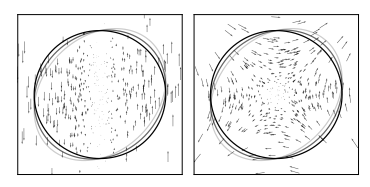
\includegraphics[width=0.35\textwidth]{figures/velocity.png}
      \caption{Velocity field}
      \label{fig:velocity}
    \end{figure}

\end{frame}

\begin{frame}
    \frametitle{Loss Function}
    \begin{block}{The Transport Equation}
    Given a solution to the equation, we can form the gradient estimator 
    $$\nabla_{\theta} \mathcal{L} = \mathbb{E}_{q_{\theta}(z)} \left[ v^{\theta} \cdot \nabla_{z} f \right].$$
    \end{block}

    \begin{block}{Tangent Fields}
    To determine a unique solution—the tangent field from the theory of optimal transport—we require that
    $$\frac{\partial v_i^{\text{OMT}}}{\partial z_j} = \frac{\partial v_j^{\text{OMT}}}{\partial z_i} \quad \forall i, j.$$
    In this case it can be shown that $\mathbf{v}^\text{OMT}$ minimizes the total kinetic energy, which is given by
    $$K(v) = \frac{1}{2} \int dz \, q_{\theta}(z) \|v\|^2 $$
    \end{block}

\end{frame}

\begin{frame}
    \frametitle{About optimal solution}
    \begin{block}{OMT is not optimal}
    The ||v||2term that appears in Eqn. 15 might lead one to hope that v OMT provides gradients that minimize gradient variance. Unfortunately, the situation is more complicated. Denoting the (mean) gradient by $\mathbf{g} = \mathbb{E}_{q_0(z)} \left[ v \cdot \nabla_z f \right] - \| g \|^2$ the total gradient variance is given by
    $$ \mathbb{E}_{q_0(z)} \left[ \| v \cdot \nabla_z f \|^2 \right] - \| g \|^2$$
    \end{block}

    \begin{block}{OMT is approximation of optimum}
    Still, for many choices of $f\mathbf{(z})$ we expect the
OMT gradient estimator to have lower variance than the RT gradient estimator, since the latter has no particular optimality guarantees (at least not in any coordinate system that we
expect to be well adapted to $f(\mathbf{z})$)).
    \end{block}

\end{frame}
\section{Numerical cases}
\begin{frame}
    \frametitle{Beta}
    \begin{figure}[h!]
      \centering
      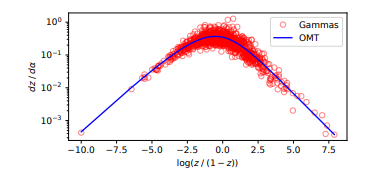
\includegraphics[width=0.38\textwidth]{figures/beta_der.png}
      \caption{Derivatives $\frac{dz}{d\alpha}$ for samples $z \sim \text{Beta}(1, 1)$. }
      \label{fig:beta_der}
    \end{figure}
    \begin{figure}[h!]
      \centering
      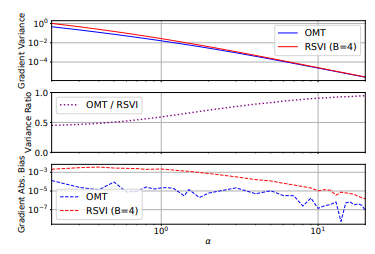
\includegraphics[width=0.38\textwidth]{figures/beta_grad.png}
      \caption{We compare the OMT gradient to the RSVI gradient with
$B = 4$ for the test function $f(z) = z^3$}
      \label{fig:beta_der}
    \end{figure}
\end{frame}
\begin{frame}
    \frametitle{Dirichlet}
    \begin{figure}[h!]
      \centering
      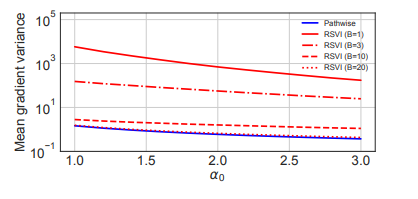
\includegraphics[width=0.8\textwidth]{figures/dirichlet.png}
      \caption{. Gradient variance for the ELBO of a conjugate
Multinomial-Dirichlet model. We compare the pathwise gradient to RSVI for different boosts B. S}
      \label{fig:dirichlet}
    \end{figure}

\end{frame}


\begin{frame}
    \frametitle{Quetions}
    TThat's all
\end{frame}
\end{document}
